\documentclass[12pt]{article}

\usepackage[a4paper,width=160mm,top=20mm,bottom=20mm,bindingoffset=6mm]{geometry}
\usepackage[utf8]{inputenc}
\usepackage[italian]{babel}
\usepackage[OT1]{fontenc}
\usepackage{graphicx}
\usepackage{float}
\usepackage{fancyhdr}
\usepackage{xcolor}
\usepackage{mathtools}
\usepackage{amsmath}
\usepackage{amssymb}
\usepackage{tikz}
\usepackage{imakeidx}
\usepackage{textcomp}
\usepackage{pifont}
\usepackage{polynom}
\usepackage{algorithm}
\usepackage{algpseudocode}
\usepackage{mathtools}
\usepackage[colorlinks=true,linkcolor=black,anchorcolor=black,citecolor=black,filecolor=black,menucolor=black,runcolor=black,urlcolor=black]{hyperref}
\usepackage{cancel}
\usepackage{pgfplots}
\usepackage{caption}
\usepackage{tabularx}
\usepackage{comment}
\usepackage{float}
\usepackage{bm}



\begin{document}
\bibliographystyle{plain}
    \pagestyle{fancy}
    \everymath{\displaystyle}
    \sffamily
    \begin{figure}
        \centering
        
\includegraphics[scale=0.1]{images/uniba-logo.png}
        \caption*{Università degli Studi di Bari Aldo Moro}
    \end{figure}
    
    \title{Relazione tecnica Sustainability of RecSys}
    \author{Emanuele Fontana}
    \date{Tirocinio tesi triennale in Informatica\\Anno accademico 2023/2024}
    \maketitle
    \tableofcontents\newpage
    \section{Introduzione}
Tracciare le emissioni degli algoritmi di raccomandazione e cercare di prevederle è molto importante quando si parla di sviluppo sostenibile in campo RecSys. Ancora oggi si tende a trascurare l'impatto ambientale di un'attività e, in questo ambito, si è molto propensi nell'utilizzare dei modelli molti complessi e pesanti
che richiedono molte risorse per essere addestrati ed eseguti per ottenere delle buone performance. Spesso, però, modelli molto più leggeri e semplici riescono a ottenere delle performance molto simili (se non superiori) a modelli più complessi e il tutto con un impatto ambientale decisamente minore.
Ad oggi il carbon dioxide equivalent (CO$_2$eq) è il principale indicatore utilizzato da governi e enti per misurare l'impatto ambientale di un'attività.
Il CO$_2$eq è un'unità di misura che esprime l'equivalente in CO$_2$ di tutti i gas serra emessi da un'attività, in modo da poter confrontare l'impatto ambientale di attività diverse.
Una strategia comune per calcolare il CO$_2$eq è quella di moltiplicare tra loro il \textbf{carbon intensity(CI)} e l'\textbf{energia consumata(PC)} dall'attività (nel nostro caso l'esecuzione di algoritmi).



\begin{equation*}
    \textit{emission} = \textit{CI}  \cdot \textit{PC}
\end{equation*}

\noindent In particolare i valori di CI dipendono dalle diverse fonti di energia utilizzate durante la computazione 
(es. energia solare, energia eolica, etc.). Se \textit{s} è la fonte di energia,  \textit{e$_s$} sono le emissioni per KW/h di energia e \textit{p$_s$}  è la percentuale di energia prodotta dalla fonte s, allora il CI è dato da:
\begin{equation*}
    \textit{CI} = \sum_{s \in S} \textit{e$_s$} \cdot \textit{p$_s$}
\end{equation*}

%give me author name of the paper spillo2023towards

\noindent Lo scopo di questo lavoro è quello di valutare e prevedere l'impatto ambientale di un sistema di raccomandazione (RecSys) in base alla sua sostenibilità. Per quanto riguarda la valutazione, mediante la libreria CodeCarbon\footnote{\href{http://codecarbon.io}{CodeCarbon}}{} è stato possibile misurare le emissioni prodotte dalla macchina durante l'addestramento con parametri di default per un dato modello dato un dataset. 
In questo ambito  Spillo et al.\cite{spillo2023towards} mostrano come spesso algoritmi più semplici riescono ad avere delle performance molto simili a modelli più complessi, ma con un impatto ambientale decisamente minore.
\begin{figure}[H]
    \centering
    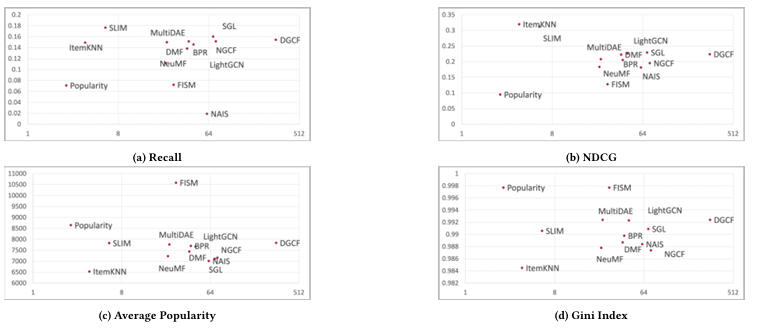
\includegraphics[scale=0.75]{images/risultati-valutazione.png}
    \caption*{Trade-off tra emissioni e performance con dataset Mind}


\end{figure}
\noindent Per quanto riguarda la previsione questo documento si propone di presentare lo stato attuale del lavoro svolto in questo ambito.
\begin{figure}[H]
    \centering
    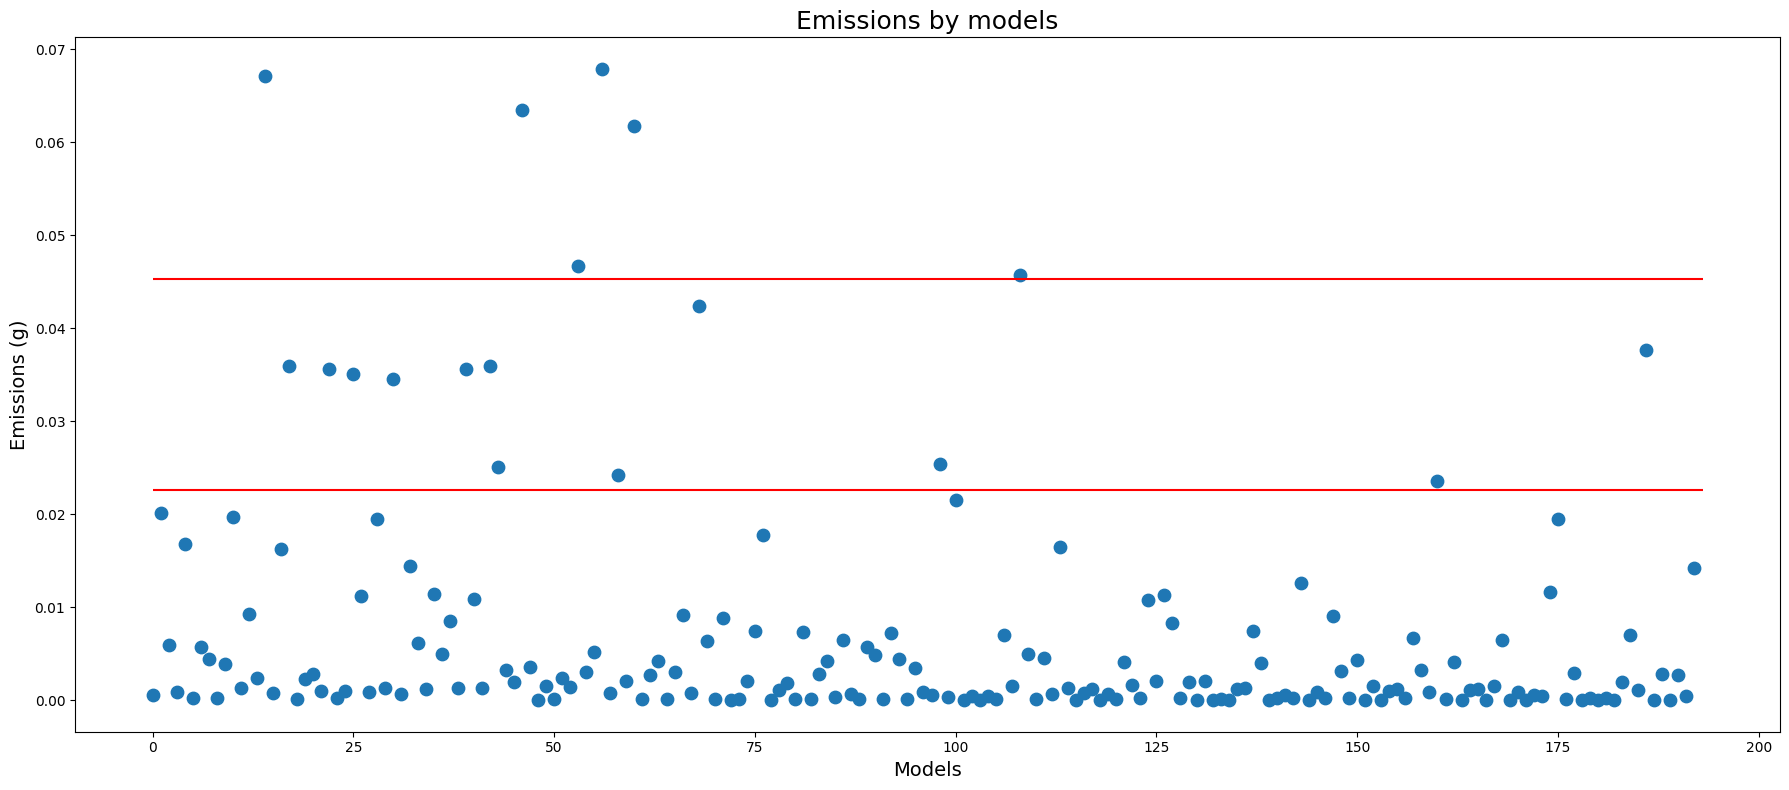
\includegraphics[scale=0.25]{images/situazione-attuale.png}
    \caption*{Emissioni prodotte dai vari modelli}
\end{figure}

\noindent L'esperimento è stato condotto su dataset presenti all'interno della libreria python RecBole\footnote{\href{http://recbole.io}{RecBole}}{}, una libreria open-source che offre un'implementazione di modelli di raccomandazione. I dataset utilizzati per l'addestramento dei modelli sono:
\begin{itemize}
    \item \textbf{MovieLens-1M}\footnote{\href{https://github.com/RUCAIBox/RecSysDatasets/blob/master/conversion_tools/usage/MovieLens.md}{Dataset MovieLens}}{}
    \item \textbf{Amazon\_Book\_60core\_kg} \footnote{\href{https://github.com/RUCAIBox/RecSysDatasets/blob/master/conversion_tools/usage/Amazon-book-KG.md}{Dataset Amazon\_Book\_60core\_kg}}{}
    \item \textbf{Mind}\footnote{\href{https://github.com/RUCAIBox/RecSysDatasets/blob/master/conversion_tools/usage/MIND.md}{Dataset MIND}}{}
\end{itemize}




    \newpage
    \section{Dataset del regressore}
In questo capitolo si analizza il dataset utilizzato e come questo è stato trattato per l'addestramento dei modelli. Inoltre, si descrivono le feature di input e output del modello.

\noindent Il dataset nella sua totalità è composto da 13 feature di input e una feature di output. Le feature di input possiamo suddividerle in 4 categorie:
\begin{itemize}
    \item \textbf{Feature relative al dataset}, quali \textit{n\_users}, \textit{n\_items}, \textit{n\_inter}, \textit{sparsity}
    \item \textbf{Feature relative al knowledge graph}, quali \textit{kg\_entities}, \textit{kg\_relations}, \textit{kg\_triples}, \textit{kg\_items}
    \item \textbf{Feature relative all'hardware utilizzato per l'addestramento}, quali \textit{cpu\_cores}, \textit{ram\_size}, \textit{is\_gpu}
    \item \textbf{Feature relative al modello}, quali \textit{model\_name}, \textit{model\_type}
\end{itemize}
Nel dataset sono presenti 201 righe (dunque 201 esperimenti distinti).
\subsection{Descrizione delle feature di output}
La feature di output \textit{emissions} rappresenta le emissioni di CO$_2$eq prodotte dalla macchina durante l'addestramento del modello.
\subsection{Descrizione delle feature di input}
\begin{center}
\begin{table}[H]
    \centering
    \begin{tabularx}{\textwidth}{|c|X|}
        \hline
        \textbf{Feature} & \textbf{Descrizione} \\
        \hline
        n\_users & Numero di utenti presenti nel dataset \\
        \hline
        n\_items & Numero di items presenti nel dataset \\
        \hline
        n\_inter & Numero di interazioni nel dataset. Per interazione si intendono le varie interazioni (valutazioni) tra gli utenti nel dataset e gli item nel dataset \\
        \hline
        sparsity & Sparsità del dataset. La sparsità indica la percentuale di valori mancanti nel dataset (quindi mancanza di interazione tra utenti e item)\\
        \hline
        kg\_entities & Numero di entità nel knowledge graph. Un'entità è un oggetto distintivo o un concetto unico all'interno del Knowledge Graph \\
        \hline
        kg\_relations & Numero di relazioni nel knowledge graph. Le relazioni rappresentano i legami o collegamenti tra le entità all'interno del Knowledge Graph. Sono spesso definite dai predicati nelle triple \\
        \hline
        kg\_triples & Numero di triple nel knowledge graph. Una triple è una struttura dati fondamentale nel Knowledge Graph che consiste in tre parti: soggetto, predicato e oggetto. Queste triple rappresentano le relazioni tra le entità \\
        \hline
        kg\_items & Numero di items nel knowledge graph. Gli "Items" nel contesto del Knowledge Graph sono gli oggetti specifici o le entità che sono inclusi nel grafo \\
        \hline
        cpu\_cores & Numero di core della CPU \\
        \hline
        ram\_size & Dimensione della RAM \\
        \hline
        is\_gpu & Booleano che indica se la macchina ha usato una GPU per l'addestramento \\
        \hline
        model\_name & Nome del modello \\
        \hline
        model\_type & Tipo del modello \\
        \hline
    \end{tabularx}
    \caption*{Descrizione delle feature di input}
\end{table}
\end{center}

Per quanto riguarda la feature \textit{model\_type} abbiamo i seguenti valori:
\begin{itemize}
    \item \textbf{General}: Modelli che si basano su tecniche tradizionali
    \item \textbf{Knowledge}: Modelli che incorporano conoscenza esterna (knowledge graph) per migliorare le raccomandazioni
\end{itemize}

Per quanto riguarda la feature \textit{model\_name} abbiamo i seguenti valori:
\begin{itemize}
    \item \textbf{BPR} \cite{BPR}: General
    \item \textbf{CDAE} \cite{CDAE}: General
    \item \textbf{CFKG} \cite{CFKG}: Knowledge
    \item \textbf{CKE} \cite{CKE}: Knowledge
    \item \textbf{DGCF} \cite{DGCF}: Knowledge
    \item \textbf{DMF} \cite{DMF}: General
    \item \textbf{DiffRec} \cite{DiffRec}: General
    \item \textbf{ENMF} \cite{ENMF}: General 
    \item \textbf{FISM} \cite{FISM}: General
    \item \textbf{GCMC} \cite{GCMC}: General
    \item \textbf{ItemKNN} \cite{ItemKNN}: General
    \item \textbf{KGCN} \cite{KGCN}: Knowledge
    \item \textbf{KGIN}: \cite{KGIN} Knowledge
    \item \textbf{KGNNLS} \cite{KGNNLS}: Knowledge
    \item \textbf{KTUP} \cite{KTUP}: Knowledge
    \item \textbf{LDiffRec} \cite{LDiffRec}: General
    \item \textbf{LINE} \cite{LINE}: General
    \item \textbf{LightGCN} \cite{LightGCN}: General
    \item \textbf{MKR} \cite{MKR}: Knowledge
    \item \textbf{MacridVAE} \cite{MacridVAE}: General
    \item \textbf{MultiDAE} \cite{MultiDAE}: General
    \item \textbf{MultiVAE} \cite{MultiVAE}: General
    \item \textbf{NCEPLRec} \cite{NCEPLRec}: General
    \item \textbf{NCL} \cite{NCL}: General
    \item \textbf{NGCF} \cite{NGCF}: General
    \item \textbf{NeuMF} \cite{NeuMF}: General
    \item \textbf{Pop}: General
    \item \textbf{Random}: General
    \item \textbf{RecVAE} \cite{RecVAE}: General
    \item \textbf{RippleNet} \cite{RippleNet}: Knowledge
    \item \textbf{SGL} \cite{SGL}: General
    \item \textbf{SLIMElastic} \cite{SLIMElastic}: General
    \item \textbf{SimpleX} \cite{SimpleX}: General
    \item \textbf{SpectralCF} \cite{SpectralCF}: General
    \item \textbf{EASE} \cite{EASE}: General
    \item \textbf{NAIS} \cite{NAIS}: General
    \item \textbf{ADMMSLIM} \cite{ADMMSLIM}: General
    \item \textbf{ConvNCF} \cite{ConvNCF}: General
    \item \textbf{NNCF} \cite{NNCF}: General
\end{itemize}

Altri valori unici presenti per le varie feature di input sono:
\begin{itemize}
    \item \textbf{n\_users}: [22155, 23679, 6040]
    \item \textbf{n\_items}: [54458, 4414, 3706]
    \item \textbf{n\_inter}: [1465871, 1048575, 1000209]
    \item \textbf{sparsity}: [0.99878504, 0.98996762, 0.95531637]
    \item \textbf{kg\_entities}: [26315, 0, 79347]
    \item \textbf{kg\_relations}: [16, 0, 49]
    \item \textbf{kg\_triples}: [96476, 0, 385923]
    \item \textbf{kg\_items}: [11446, 0, 3655]
    \item \textbf{cpu\_cores}: [12, 4]
    \item \textbf{ram\_size}: [64, 16, 27.40581512]
    \item \textbf{is\_gpu}: [1, 0]
\end{itemize}
\subsection{Pre-Processing}

Per poter sfruttare le feature di input per l'addestramento del modello, è stato necessario effettuare un pre-processing. Le feature \textit{model\_name} e \textit{model\_type} sono state trasformate in variabili numeriche. In particolare il valore \textit{general} è stato trasformato in 0 e il valore \textit{knowledge} è stato trasformato in 1.
Per quanto riguarda la feature \textit{model\_name}, ogni valore è stato trasformato in un numero intero univoco. In questo modo, il modello può sfruttare queste feature per l'addestramento.
Prima di cominciare con l'addestramento dei modelli la feature di output è stata separata dalle feature di input. I dati sono poi stati suddivisi rispettivamente in training set e test set. In particolare il 70\% dei dati è stato usato per l'addestramento, mentre il 30\% è stato usato per la valutazione. Inoltre, mediante il \textit{random\_state}=2, è garantita la riproducibilità dell'esperimento.


    \newpage
    \section{Modelli di regressione}
\subsection{Introduzione ai regressori}
I regressori sono dei modelli di machine learning il cui obiettivo è quello di prevedere un valore numerico continuo (in questo caso il valore delle emissioni).
I regressori vengono valutati sulla base di metriche quali, per esempio, l'errore quadratico medio (MSE), l'errore assoluto medio (MAE), e l'errore quadrato logaritmico medio (MSLE).

\subsection{Regressori utilizzati}
In questo lavoro sono stati utilizzati i seguenti regressori:
\begin{itemize}
    \item \textbf{Support Vector Regression (SVR)}\footnote{\href{https://scikit-learn.org/stable/modules/generated/sklearn.svm.SVR.html}{SVR}}{}
    \item \textbf{Decision Tree Regressor} \footnote{\href{https://scikit-learn.org/stable/modules/generated/sklearn.tree.DecisionTreeRegressor.html}{Decision Tree Regressor}}{}
    \item \textbf{Random Forest Regressor} \footnote{\href{https://scikit-learn.org/stable/modules/generated/sklearn.ensemble.RandomForestRegressor.html}{Random Forest Regressor}}{}
    \item \textbf{AdaBoost Regressor} \footnote{\href{https://scikit-learn.org/stable/modules/generated/sklearn.ensemble.AdaBoostRegressor.html}{AdaBoost Regressor}}{}
\end{itemize}
\subsubsection{Support Vector Regression (SVR)}
%add a footnote to SVM
La SVR è un algoritmo che estende il concetto di Support Vector Machine (SVM)\footnote{Algoritmi di classificazione che cercano di trovare un iperpiano ottimale per ottenere separabilità lineare}{} al caso della regressione.
\begin{figure}[H]
    \centering
    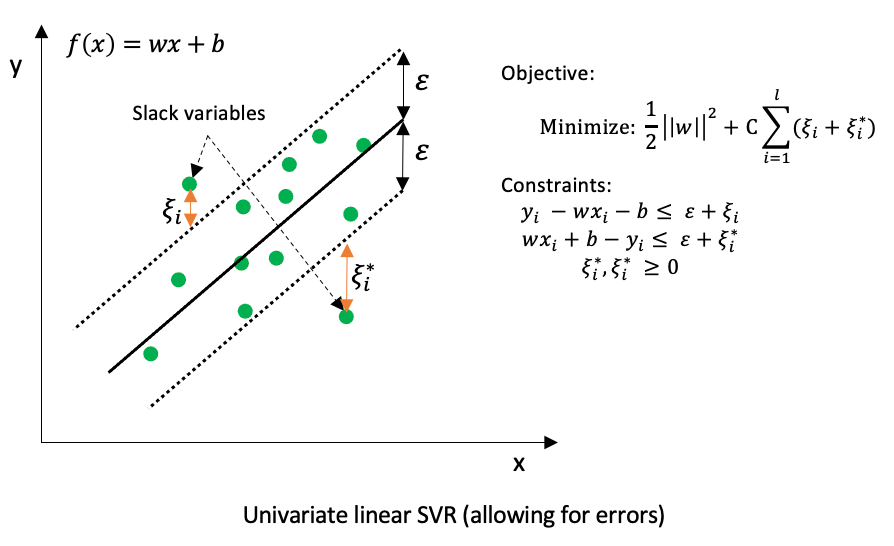
\includegraphics[scale=0.5]{images/SVR.png}
    \caption*{Esempio di SVR}
\end{figure} \newpage
\noindent In questo lavoro il modello è stato costruito usando gli iperparametri di default. Questi ultimi sono:
\begin{itemize}
    \item \textbf{kernel=rbf}: E' il tipo di Kernel\footnote{Funzione matematica usata per mappare i dati originali in uno spazio di dimensione superiore}{} utilizzato. Questo kernel valuta quanto due punti siano simili sulla base della loro distanza
    \item \textbf{degree=3}:  grado del polinomio utilizzato per la trasformazione dei dati nello spazio
    \item \textbf{gamma=scale}: coefficiente del kernel
    \item \textbf{coef0=0.0}: termine indipendente nel kernel
    \item \textbf{tol=0.001}: tolleranza per il criterio di arresto
    \item \textbf{C=1.0}: parametro di regolarizzazione
    \item \textbf{epsilon=0.1}:  controlla la tolleranza del modello nei confronti degli errori nella predizione
    \item \textbf{shrinking=True}: se abilitare o meno la riduzione del set di supporto
    \item \textbf{cache\_size=200}: dimensione della cache in MB
    \item \textbf{max\_iter=-1}: numero massimo di iterazioni. -1 indica nessun limite
\end{itemize}


\subsubsection{Decision Tree Regressor}

I Decision Tree Regressors sono modelli di regressione basati su alberi decisionali. Questi algoritmi suddividono ripetutamente il set di dati in base alle caratteristiche (features) per creare una struttura ad albero che rappresenta la relazione di decisione. Ogni nodo interno dell'albero rappresenta una decisione basata su una caratteristica, e le foglie dell'albero contengono i valori di output previsti.
\begin{figure}[H]
    \centering
    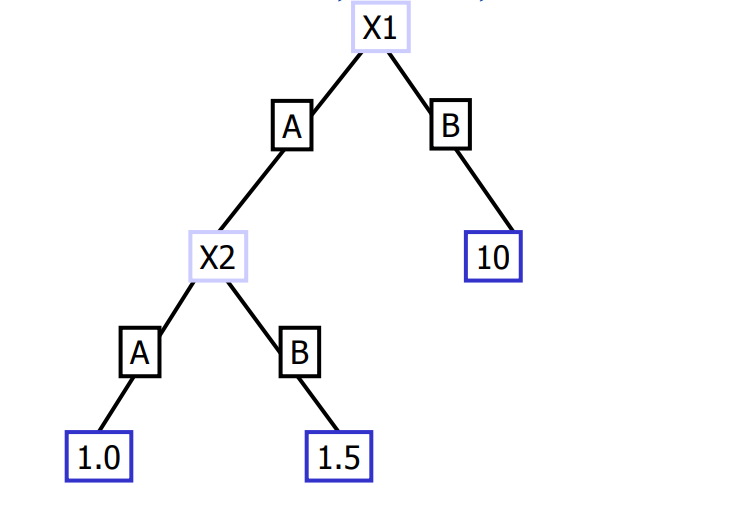
\includegraphics[scale=0.5]{images/DecisionTreeRegressor.png}
    \caption*{Esempio di albero decisionale di regressione}
\end{figure}

\noindent In questo lavoro due iperparametri sono stati decisi all'atto della costruzione del modello:
\begin{itemize}
    \item \textbf{max\_depth=5}: profondità massima dell'albero
    \item \textbf{random\_state=3}:  controlla la casualità nell'addestramento del modello. Quando viene fissato a un numero intero specifico l'addestramento del modello sarà deterministico, cioè produrrà gli stessi risultati in ogni esecuzione
\end{itemize}
\noindent mentre gli altri iperparametri sono stati lasciati ai valori di default:
\begin{itemize}
    \item \textbf{criterion=squared\_error}: Criterio per stabilire la qualità di una suddivisione
    \item \textbf{splitter=best}: Strategia per scegliere la suddivisione in ogni nodo
    \item \textbf{min\_samples\_split=2}: Numero minimo di campioni richiesti per suddividere un nodo interno
    \item \textbf{min\_samples\_leaf=1}: Numero minimo di campioni richiesti per essere in una foglia
    \item \textbf{min\_weight\_fraction\_leaf=0.0}: La frazione minima dei campioni totali (pesati) necessaria affinché si verifichi un nodo foglia
    \item \textbf{max\_features=None}: Numero di features da considerare quando si cerca la migliore suddivisione. None indica tutte
    \item \textbf{max\_leaf\_nodes=None}: Numero massimo di foglie. None indica nessun limite
    \item \textbf{min\_impurity\_decrease=0.0}: Un nodo verrà suddiviso se questa suddivisione induce una diminuzione dell'impurità maggiore o uguale a questo valore
    \item \textbf{ccp\_alpha=0.0}: Parametro di complessità usato per la potatura
    \item \textbf{monotonic\_constraints=None}: Vincoli monotoni sui valori delle features
\end{itemize}

\subsubsection{Random Forest Regressor}
I Random Forest Regressors sono modelli di regressione basati su alberi decisionali. Vengono costruiti su più alberi decisionali che combinano le loro previsioni per ottenere una previsione più accurata e stabile.
\begin{figure}[H]
    \centering
    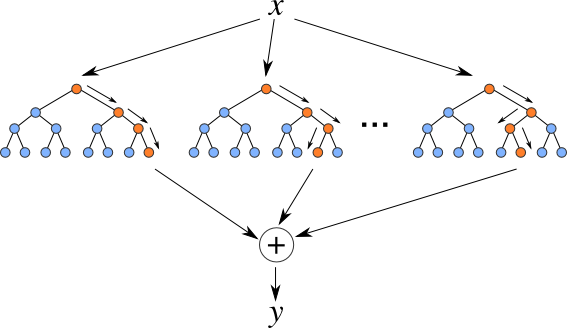
\includegraphics[scale=0.5]{images/RandomForestRegressor.png}
    \caption*{Esempio di Random Forest Regresor}
\end{figure}

\noindent In questo lavoro tre iperparametri sono stati decisi all'atto della costruzione del modello:
\begin{itemize}
    \item \textbf{n\_estimators=500}: numero di alberi nella foresta
    \item \textbf{max\_depth=5}: profondità massima dell'albero
    \item \textbf{random\_state=3}:  controlla la casualità nell'addestramento del modello. Quando viene fissato a un numero intero specifico l'addestramento del modello sarà deterministico, cioè produrrà gli stessi risultati in ogni esecuzione
\end{itemize}

\noindent mentre gli altri iperparametri sono stati lasciati ai valori di default:
\begin{itemize}
    \item \textbf{criterion=squared\_error}: Criterio per stabilire la qualità di una suddivisione
    \item \textbf{min\_samples\_split=2}: Numero minimo di campioni richiesti per suddividere un nodo interno
    \item \textbf{min\_samples\_leaf=1}: Numero minimo di campioni richiesti per essere in una foglia
    \item \textbf{min\_weight\_fraction\_leaf=0.0}: La frazione minima dei campioni totali (pesati) necessaria affinché si verifichi un nodo foglia
    \item \textbf{max\_features=1}: Numero di features da considerare quando si cerca la migliore suddivisione
    \item \textbf{max\_leaf\_nodes=None}: Numero massimo di foglie. None indica nessun limite
    \item \textbf{min\_impurity\_decrease=0.0}: Un nodo verrà suddiviso se questa suddivisione induce una diminuzione dell'impurità maggiore o uguale a questo valore
    \item \textbf{ccp\_alpha=0.0}: Parametro di complessità usato per la potatura
    \item \textbf{bootstrap=True}: Se utilizzare il bootstrap per la costruzione degli alberi
    \item \textbf{oob\_score=False}: Se calcolare l'errore out-of-bag
    \item \textbf{n\_jobs=None}: Numero di lavori da eseguire in parallelo. None indica 1
    \item \textbf{warm\_start=False}: Se utilizzare la soluzione precedente come inizializzazione
    \item \textbf{max\_samples=None}: Numero massimo di campioni da utilizzare per la costruzione di ciascun albero. None indica tutti
    \item \textbf{monotonic\_constraints=None}: Vincoli monotoni sui valori delle features
\end{itemize}
\newpage
\subsubsection{AdaBoost Regressor}
L'AdaBoost Regressor è un modello basato sull'algoritmo di boosting AdaBoost\footnote{Crea un modello forte combinando modelli più deboli, ognuno allenato su diverse parti del dataset}{}. Questo algoritmo costruisce un modello di previsione combinando più modelli di previsione più deboli.
\begin{figure}[H]
    \centering
    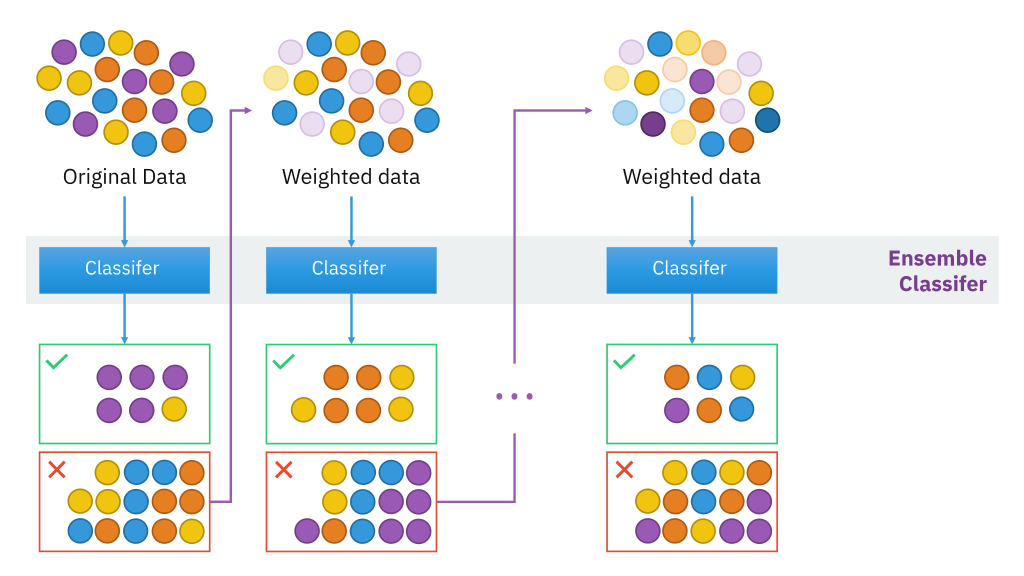
\includegraphics[scale=0.4]{images/AdaBoost.png}
    \caption*{Struttura di modello basato su AdaBoost}
\end{figure}

\noindent In questo lavoro due iperparametri sono stati decisi all'atto della costruzione del modello:

\begin{itemize}
    \item \textbf{n\_estimators=500}: numero di stimatori
    \item \textbf{random\_state=3}:  controlla la casualità nell'addestramento del modello. Quando viene fissato a un numero intero specifico l'addestramento del modello sarà deterministico, cioè produrrà gli stessi risultati in ogni esecuzione
\end{itemize}

\noindent mentre gli altri iperparametri sono stati lasciati ai valori di default:
\begin{itemize}
    \item \textbf{estimator=None}: stimatore base. Se None, viene utilizzato DecisionTreeRegressor
    \item \textbf{learning\_rate=1.0}: tasso di apprendimento
    \item \textbf{loss=linear}: funzione di perdita
\end{itemize}


    \newpage
    \section{Risultati}

In questo capitolo si analizzano i risultati degli esperimenti che sono stati condotti. I regressori utilizzati sono stati valutati utilizzando le seguenti metriche per la regressione:
\begin{itemize}
    %add the mathematic formula of each error
    \item \textbf{Mean Absolute Error (MAE)}: è la media della differenza assoluta tra le previsioni e i valori reali.
    \begin{equation*}
        MAE = \frac{1}{n} \sum_{i=1}^{n} |y_i - \hat{y}_i|
    \end{equation*}
    \item \textbf{Root Mean Squared Error (RMSE)}: è la radice quadrata della media della differenza tra le previsioni e i valori reali al quadrato.
    \begin{equation*}
        RMSE = \sqrt{\frac{1}{n} \sum_{i=1}^{n} (y_i - \hat{y}_i)^2}
    \end{equation*}
    \item \textbf{Mean Logarithmic Squared Error (MSLE)}: è la media del logaritmo dei quadrati degli errori.
    \begin{equation*}
        MSLE = \frac{1}{n} \sum_{i=1}^{n} (\log(y_i + 1) - \log(\hat{y}_i + 1))^2
    \end{equation*}
\end{itemize}

\subsection{Risultati ottenuti}

\begin{table}[H]
    \centering
    \begin{tabular}{|>{\centering\arraybackslash}m{5cm}|c|c|c|c|}
        \hline
        \textbf{Regressor} & \textbf{MAE} & \textbf{RMSE} & \textbf{MSLE} \\ [10pt]
        \hline
        SVR & 0.0288215 & 0.0008862 & 0.0008537 \\ [10pt]
        \hline
        Decision Tree & 0.0048531 & 0.0000969 & 0.0000918 \\ [10pt]
        \hline
        Random Forest & 0.0054369 & 0.0001088 & 0.0001026 \\ [10pt]
        \hline
        AdaBoost & 0.0071778 & 0.0001113 & 0.0001059 \\ [10pt]
        \hline
    \end{tabular}
    \caption*{Risultati ottenuti}
    \label{tab:results}
\end{table}

\begin{table}[H]
    \centering
    \begin{tabular}{c c}
        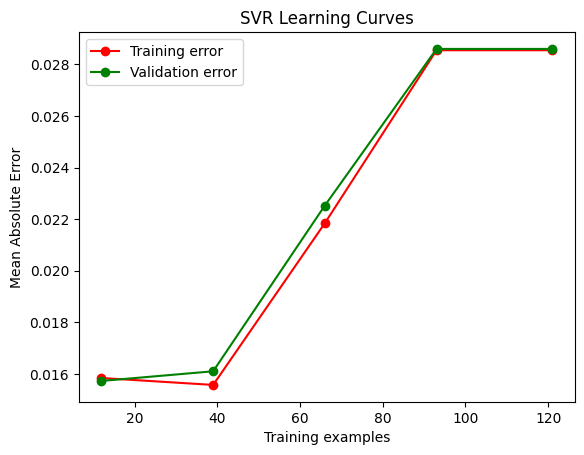
\includegraphics[scale=0.3]{images/SVR_lc.png} & 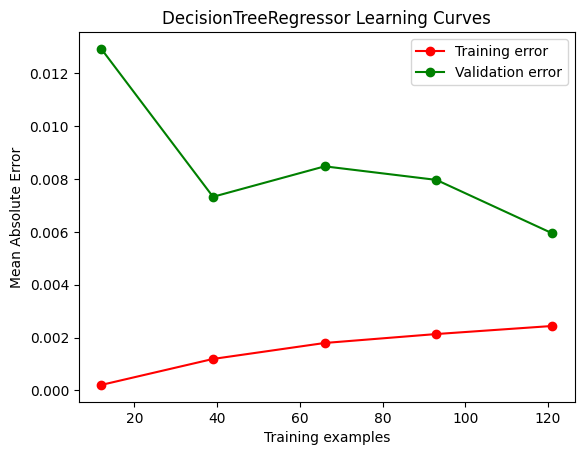
\includegraphics[scale=0.3]{images/DecisionTree_lc.png} \\
        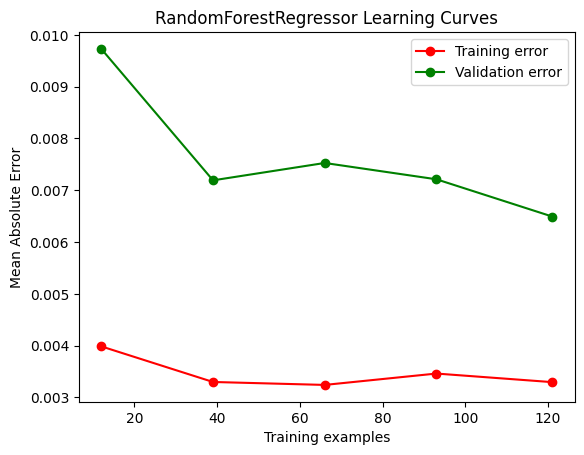
\includegraphics[scale=0.3]{images/RandomForestRegressor_lc.png} & 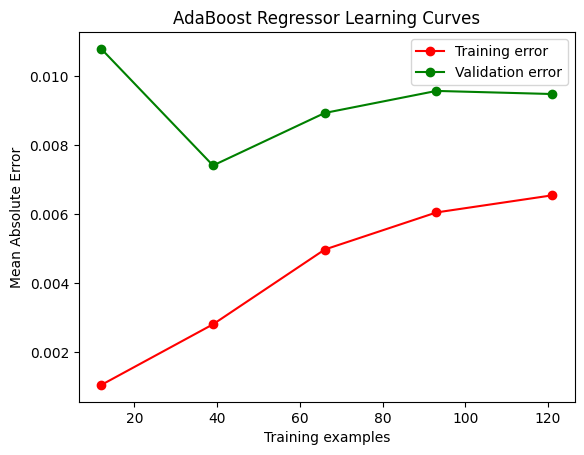
\includegraphics[scale=0.3]{images/AdaBoostRegressor_lc.png} \\
    \end{tabular}
    \caption*{Learning curve dei regressori}
    \label{tab:lc}
\end{table}

\subsection{Analisi dei risultati}


    \paragraph{\textbf{SVR}.}
    Dal punto di vista delle metriche il regressore SVR ha ottenuto i peggiori risultati in termini di MAE, RMSE e MSLE. La learning curve mostra che il modello è in overfitting, infatti gli errori aumentano all'aumentare del numero di istanze.
   
   
    \paragraph{\textbf{Decision Tree Regressor}.}
    Dal punto di vista delle metriche, il Decision Tree Regressor ha ottenuto i migliori risultati. 
    La learning curve mostra una curva di training che aumenta all'aumentare del numero di istanze, mentre la curva di validation diminuisce. Le due curve si avvicinano, ma non si sovrappongono. Sembra esserci un leggero underfitting.
    \paragraph{\textbf{Random Forest Regressor}.}
    Dal punto di vista delle metriche il Random Forest Regressor risulta essere il secondo miglior modello.
    La learning curves di train e di validation set diminuiscono entrambe all'aumentare del numero di istanze, ma non si sovrappongono. Anche qui sembra esserci underfitting.
    \paragraph{\textbf{AdaBoost Regressor}.}
    Dal punto di vista delle metriche il AdaBoost Regressor ha ottenuto risultati peggiori rispetto al Random Forest Regressor ma migliori rispetto al SVR.
    La learning curve mostrano che il modello non è riuscito a generalizzare bene


\subsection{Conclusioni}
Il dataset sembra essere troppo piccolo per poter generalizzare bene i modelli. Inoltre, il dataset è molto sbilanciato, con pochi valori per ogni feature. Questo potrebbe essere un motivo per cui i modelli non generalizzano bene. Inoltre, i modelli non sono stati ottimizzati, quindi potrebbero essere migliorati mediante ricerca di iperparametri.
Per i risultati attuali, il Decision Tree Regressor è il modello migliore.
    \newpage
    
    \section{Statistiche dei dataset}

LFM1b\_artist è un dataset contenente informazioni riguardanti le interazioni tra utenti e artisti musicali.



\subsection{Dataset originale}


Descrizione del dataset
\begin{table}[H]
    \centering
    \footnotesize
    \begin{tabularx}{\textwidth}{|c|X|}
        \hline
        \textbf{Feature} & \textbf{Descrizione} \\
        \hline
        n\_users & 120322 \\
        \hline
        n\_items & 3123496 \\
        \hline
        n\_inter & 65133026 \\
        \hline
        sparsity & 0.9998266933373666 \\
        \hline
        avg\_inter\_user & 541.3226675088513 \\
        \hline
    \end{tabularx}
    \caption{Informazioni sul dataset LFM1b\_artist}
    \label{tab:dataset_info}
\end{table}


\noindent Descrizione del knowledge graph
\begin{table}[H]
    \centering
    \footnotesize
    \begin{tabularx}{\textwidth}{|c|X|}
        \hline
        n\_ent\_head & 823213 \\
        \hline
        n\_ent\_tail & 353607 \\
        \hline
        n\_rel & 8 \\
        \hline
        n\_triple & 2114049 \\
        \hline
    \end{tabularx}
    \caption{Informazioni sul knowledge graph del dataset LFM1b\_artist}
    \label{tab:dataset_info}
\end{table}

\noindent I nomi delle relazioni presenti nel knowledge graph sono i seguenti:
\begin{itemize}
    \item music.recording.artist
    \item music.recording.releases
    \item music.recording.producer
    \item music.recording.engineer
    \item music.recording.featured\_artists
    \item music.featured\_artist.recordings
    \item music.release.artist
    \item music.artist.release
\end{itemize}

\subsection{Processing del dataset}

\subsubsection{Descrizione procedimento}

\noindent Il dataset originale risultava essere troppo grande per le risorse a nostra disposizione, dunque è stato opportunamente processato. In paritcolare sono state svolte le seguenti operazioni
\begin{itemize}
    \item \textbf{Filtraggio:} il dataset è stato filtrato eliminando tutte le interazioni in cui erano coinvolti utenti e/o item con meno di 5 interazioni
    \item \textbf{Sampling:} dopo la fase di filtraggio, è stato effettuato un sampling casuale il cui scopo era quello di ridurre il numero di utenti e di item presenti. In particolare sono stati selezionati casualmente 20000 utenti e 50000 item e sono state mantenute solo le interazioni in cui erano coinvolti utenti e item selezionati
\end{itemize}

\noindent In questo modo è stato ottenuto un dataset più piccolo e più facilmente gestibile rispetto a quello originale.
Per poter lavorare su più dataset si è deciso di effettuare un ulteriore processing del dataset, andando a creare dei sampling con una strategia di stratificazione: \footnote{{{Mantenendo il numero di utenti inalterato per ognuno di essi sono stati campionati casualmente un determinato numero di interazioni cercando di mantenere inalterati i "rapporti originali" tra i diversi utenti}}}{}
\begin{itemize}
    \item \textbf{75\%:} Per ogni utente sono state mantenute il 75\% delle interazioni originali
    \item \textbf{50\%:} Dal dataset al 75\% sono state mantenute circa il 66.67\% delle interazioni di ogni utente, in modo tale da avere il 50\% delle interazioni originali
    \item \textbf{25\%:} Dal dataset al 50\% sono state mantenute il 50\% delle interazioni di ogni utente, in modo tale da avere il 25\% delle interazioni originali
\end{itemize}

\subsubsection{Dataset core5}

Descrizione del dataset
\begin{table}[H]
    \centering
    \footnotesize
    \begin{tabularx}{\textwidth}{|c|X|}
        \hline
        \textbf{Feature} & \textbf{Descrizione} \\
        \hline
        n\_users & 120175 \\
        \hline
        n\_items & 585095 \\
        \hline
        n\_inter & 61534450 \\
        \hline
        sparsity & 0.9991248594539152 \\
        \hline
        avg\_inter\_user & 512.0403578115248 \\
        \hline
    \end{tabularx}
    \caption{Informazioni sul dataset LFM1b\_artist\_core5}
    \label{tab:dataset_info}
\end{table}


\noindent Descrizione del knowledge graph
\begin{table}[H]
    \centering
    \footnotesize
    \begin{tabularx}{\textwidth}{|c|X|}
        \hline
        n\_ent\_head & 823213 \\
        \hline
        n\_ent\_tail & 353607 \\
        \hline
        n\_rel & 8 \\
        \hline
        n\_triple & 2114049 \\
        \hline
    \end{tabularx}
    \caption{Informazioni sul knowledge graph del dataset LFM1b\_artist\_core5}
    \label{tab:dataset_info}
\end{table}

\noindent I nomi delle relazioni presenti nel knowledge graph sono i seguenti:
\begin{itemize}
    \item music.recording.artist
    \item music.recording.releases
    \item music.recording.producer
    \item music.recording.engineer
    \item music.recording.featured\_artists
    \item music.featured\_artist.recordings
    \item music.release.artist
    \item music.artist.release
\end{itemize}



\subsubsection{Dataset 20.000 users, 50.000 items}

Descrizione del dataset
\begin{table}[H]
    \centering
    \footnotesize
    \begin{tabularx}{\textwidth}{|c|X|}
        \hline
        \textbf{Feature} & \textbf{Descrizione} \\
        \hline
        n\_users & 19841 \\
        \hline
        n\_items & 42457 \\
        \hline
        n\_inter & 900212 \\
        \hline
        sparsity & 0.9989313587429705 \\
        \hline
        avg\_inter\_user & 45.371301849705155 \\
        \hline
    \end{tabularx}
    \caption{Informazioni sul dataset LFM1b\_artist\_20U50I}
    \label{tab:dataset_info}
\end{table}


\noindent Descrizione del knowledge graph
\begin{table}[H]
    \centering
    \footnotesize
    \begin{tabularx}{\textwidth}{|c|X|}
        \hline
        n\_ent\_head & 15509 \\
        \hline
        n\_ent\_tail & 35156 \\
        \hline
        n\_rel & 5 \\
        \hline
        n\_triple & 46827 \\
        \hline
    \end{tabularx}
    \caption{Informazioni sul knowledge graph del dataset LFM1b\_artist\_20U50I}
    \label{tab:dataset_info}
\end{table}

\noindent I nomi delle relazioni presenti nel knowledge graph sono i seguenti:
\begin{itemize}
    \item music.recording.artist
    \item music.recording.releases
    \item music.recording.producer
    \item music.recording.engineer
    \item music.recording.featured\_artists
\end{itemize}



\subsubsection{Dataset 75\%}

Descrizione del dataset
\begin{table}[H]
    \centering
    \footnotesize
    \begin{tabularx}{\textwidth}{|c|X|}
        \hline
        \textbf{Feature} & \textbf{Descrizione} \\
        \hline
        n\_users & 19841 \\
        \hline
        n\_items & 38932 \\
        \hline
        n\_inter & 667850 \\
        \hline
        sparsity & 0.9991354130849345 \\
        \hline
        avg\_inter\_user & 33.660097777329774 \\
        \hline
    \end{tabularx}
    \caption{Informazioni sul dataset LFM1b\_artist\_20U50I\_75strat}
    \label{tab:dataset_info}
\end{table}


\noindent Descrizione del knowledge graph
\begin{table}[H]
    \centering
    \footnotesize
    \begin{tabularx}{\textwidth}{|c|X|}
        \hline
        n\_ent\_head & 14327 \\
        \hline
        n\_ent\_tail & 32981 \\
        \hline
        n\_rel & 5 \\
        \hline
        n\_triple & 43559 \\
        \hline
    \end{tabularx}
    \caption{Informazioni sul knowledge graph del dataset LFM1b\_artist\_20U50I\_75strat}
    \label{tab:dataset_info}
\end{table}

\noindent I nomi delle relazioni presenti nel knowledge graph sono i seguenti:
\begin{itemize}
    \item music.recording.artist
    \item music.recording.releases
    \item music.recording.producer
    \item music.recording.engineer
    \item music.recording.featured\_artists
\end{itemize}



\subsubsection{Dataset 50\%}

Descrizione del dataset
\begin{table}[H]
    \centering
    \footnotesize
    \begin{tabularx}{\textwidth}{|c|X|}
        \hline
        \textbf{Feature} & \textbf{Descrizione} \\
        \hline
        n\_users & 19841 \\
        \hline
        n\_items & 33653 \\
        \hline
        n\_inter & 440620 \\
        \hline
        sparsity &  0.9993401019218887 \\
        \hline
        avg\_inter\_user & 22.20755002268031 \\
        \hline
    \end{tabularx}
    \caption{Informazioni sul dataset LFM1b\_artist\_20U50I\_50strat}
    \label{tab:dataset_info}
\end{table}


\noindent Descrizione del knowledge graph
\begin{table}[H]
    \centering
    \footnotesize
    \begin{tabularx}{\textwidth}{|c|X|}
        \hline
        n\_ent\_head & 12522 \\
        \hline
        n\_ent\_tail & 29509 \\
        \hline
        n\_rel & 5 \\
        \hline
        n\_triple & 38491 \\
        \hline
    \end{tabularx}
    \caption{Informazioni sul knowledge graph del dataset LFM1b\_artist\_20U50I\_50strat}
    \label{tab:dataset_info}
\end{table}

\noindent I nomi delle relazioni presenti nel knowledge graph sono i seguenti:
\begin{itemize}
    \item music.recording.artist
    \item music.recording.releases
    \item music.recording.producer
    \item music.recording.engineer
    \item music.recording.featured\_artists
\end{itemize}



\subsubsection{Dataset 25\%}

Descrizione del dataset
\begin{table}[H]
    \centering
    \footnotesize
    \begin{tabularx}{\textwidth}{|c|X|}
        \hline
        \textbf{Feature} & \textbf{Descrizione} \\
        \hline
        n\_users & 19841 \\
        \hline
        n\_items & 24878 \\
        \hline
        n\_inter & 218457 \\
        \hline
        sparsity & 0.9995574249320202 \\
        \hline
        avg\_inter\_user & 11.01038254120256 \\
        \hline
    \end{tabularx}
    \caption{Informazioni sul dataset LFM1b\_artist\_20U50I\_25strat}
    \label{tab:dataset_info}
\end{table}


\noindent Descrizione del knowledge graph
\begin{table}[H]
    \centering
    \footnotesize
    \begin{tabularx}{\textwidth}{|c|X|}
        \hline
        n\_ent\_head & 9444 \\
        \hline
        n\_ent\_tail & 23463 \\
        \hline
        n\_rel & 5 \\
        \hline
        n\_triple & 29822 \\
        \hline
    \end{tabularx}
    \caption{Informazioni sul knowledge graph del dataset LFM1b\_artist\_20U50I\_25strat}
    \label{tab:dataset_info}
\end{table}

\noindent I nomi delle relazioni presenti nel knowledge graph sono i seguenti:
\begin{itemize}
    \item music.recording.artist
    \item music.recording.releases
    \item music.recording.producer
    \item music.recording.engineer
    \item music.recording.featured\_artists
\end{itemize}
    \newpage
    \section{Configurazione}

\subsection{Parametri di running}
Qui di seguito vengono riportati i parametri di running dei vari esperimenti effettuati.
\subsubsection*{Parametri di environment}
I parametri di environment servono per configurare l'ambiente di esecuzione.
\begin{itemize}
    \item \textbf{gpu\_id}: 0
    \item \textbf{worker}: 0
    \item \textbf{use\_gpu}: True
    \item \textbf{seed}: 2020
    \item \textbf{state}: INFO
    \item \textbf{encoding}: utf-8
    \item \textbf{reproducibility}: True
    \item \textbf{shuffle}: True
\end{itemize}

\subsubsection*{Parametri di training}
I parametri di training servono per l'addestramento dei modelli.
\begin{itemize}
    \item \textbf{epochs}: 200
    \item \textbf{train\_batch\_size}: 2048
    \item \textbf{learner}: adam
    \item \textbf{learning\_rate}: .001
    \item \textbf{train\_neg\_sample\_args}: 
    \begin{itemize}
        \item \textbf{distribution}: uniform
        \item \textbf{sample\_num}: 1
        \item \textbf{dynamic}: False
        \item \textbf{candidate\_num}: 0
    \end{itemize}
    \item \textbf{eval\_step}: 1
    \item \textbf{stopping\_step}: 10
    \item \textbf{clip\_grad\_norm}: None
    \item \textbf{loss\_decimal\_place}: 4
    \item \textbf{weight\_decay}: .0
    \item \textbf{require\_pow}: False
    \item \textbf{enable\_amp}: False
    \item \textbf{enable\_scaler}: False
\end{itemize}

\subsubsection*{Parametri di evaluation}
I parametri di evaluation servono per valutare i modelli.
\begin{itemize}
    \item \textbf{eval\_args}:
    \item \begin{itemize}
                \item \textbf{group\_by}: user
                \item \textbf{order}: RO
                \item \textbf{split}: RS : [0.8, 0.1, 0.1]
                \item \textbf{mode}: full
            \end{itemize}
    \item \textbf{repeatable}: False
    \item \textbf{metrics}: ['Recall', 'MRR', 'NDCG', 'Hit', 'MAP', 'Precision', 'GAUC', 'ItemCoverage', 'AveragePopularity', 'GiniIndex', 'ShannonEntropy', 'TailPercentage']
    \item \textbf{topk}: 10
    \item \textbf{valid\_metric}: MRR@10
    \item \textbf{eval\_batch\_size}: 4096
    \item \textbf{metric\_decimal\_place}: 4
\end{itemize}

\subsubsection*{Iper parametri dei modelli}
Gli iper parametri dei modelli sono un insieme di parametri che vengono utilizzati per configurare i modelli. La loro configurazione può influenzare il risultato finale. Esistono delle tecniche di HyperTuning che permettono di trovare i migliori iper parametri per un determinato modello e dataset.
In questo caso si è scelto di utilizzare gli iper parametri di default



    \newpage
    \section{Emissioni}

Qui di seguito vengono riportate le emissioni di CO2 per ogni esperimento effettuato.

\begin{table}[H]
    \centering
    \footnotesize
    \setlength\tabcolsep{0pt}
    \begin{tabularx}{\textwidth}{|X|X|}
        \hline
        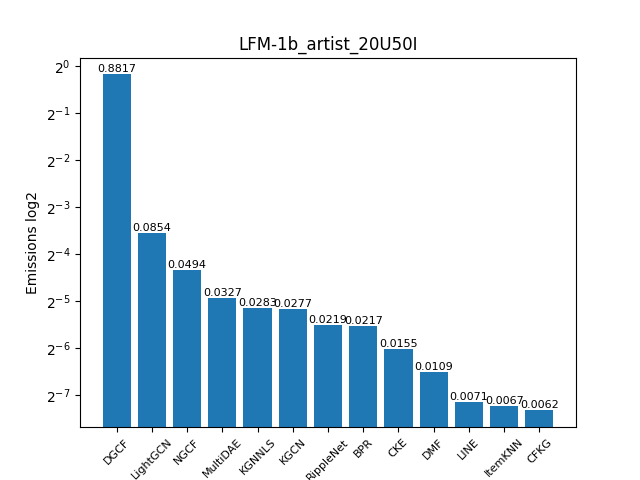
\includegraphics[width=\linewidth, trim=0 0 0 0]{images/emissions_LFM-1b_artist_20U50I.png} &
        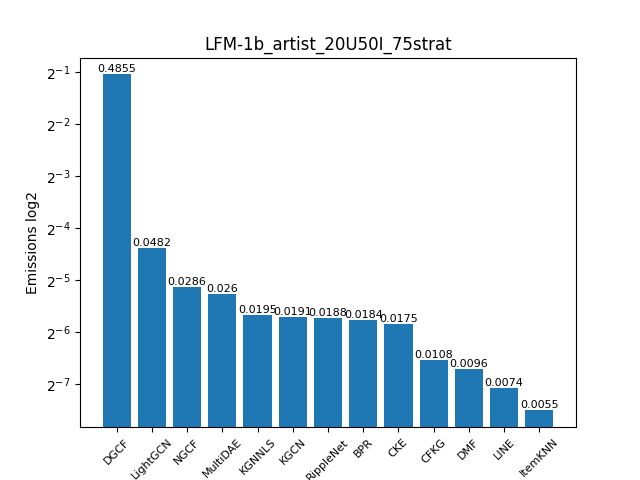
\includegraphics[width=\linewidth, trim=0 0 0 0]{images/emissions_LFM-1b_artist_20U50I_75strat.png} \\
        \hline
        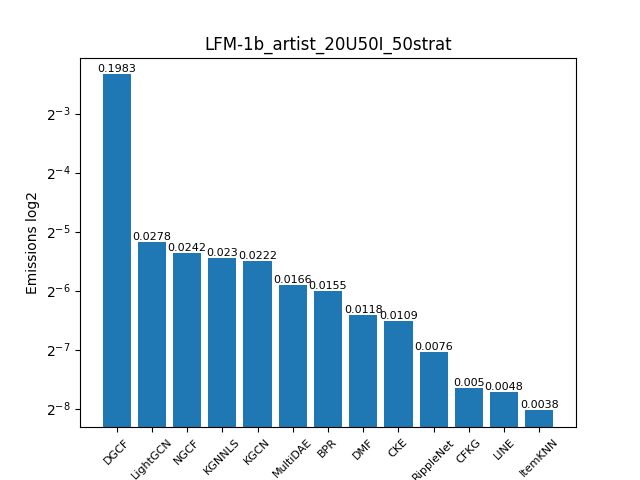
\includegraphics[width=\linewidth, trim=0 0 0 0]{images/emissions_LFM-1b_artist_20U50I_50strat.png} &
        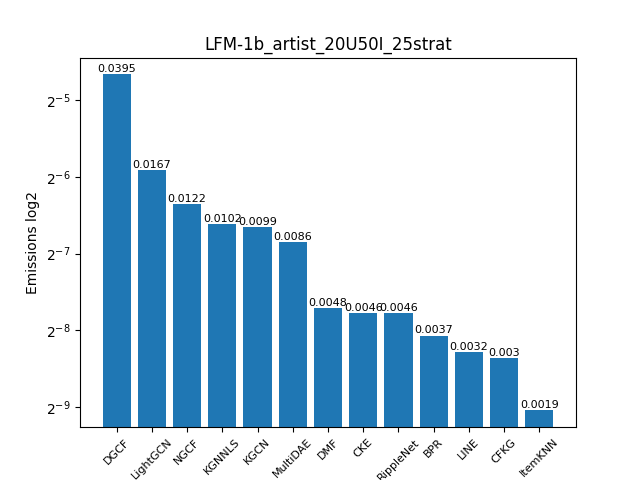
\includegraphics[width=\linewidth, trim=0 0 0 0]{images/emissions_LFM-1b_artist_20U50I_25strat.png} \\
        \hline
    \end{tabularx}
    \caption{Emissioni di CO2 per i vari dataset}
    \label{tab:emissions_info}
\end{table}

\noindent Si può subito notare come DGCF è il modello che emette più CO2 in assoluto.
In particolare con il dataset al 100\% e al 75\% DGCF emette circa 10 volte di più rispetto a LightGCN (il secondo per emissioni)
mentre con il dataset al 50\% emette circa 7 volte di più e con il dataset al 25\% emette circa 2 volte di più (sempre rispetto a LightGCN).
LightGCN e NCFG sono rispettivamente il secondo e il terzo modello che emettono più CO2.
Questi due modelli sono invece di tipo general, ma nonostante ciò emettono di più rispetto ad altri di tipo knowledge-aware, come per esempio il KGCN.
In generale possiamo vedere che ItemKNN,LINE e CFKG sono i modelli che emettono meno.
Per LINE e ItemKNN questo era abbastanza prevedibile in quanto modelli di tipo General. Interessante invece notare come CFKG, di tipo knowledge-aware, emetta meno di altri modelli di tipo General






    \newpage
    \section{Trade-off}


\subsection{Introduzione}
In questa sezione verranno analizzati i trade-off tra le varie metriche di valutazione e le emissioni di CO2 analizzando un dataset per volta.

Di seguito un elenco delle metriche con una piccola descrizione:
\begin{itemize}
    \item Recall: è una metrica che misura la capacità di un modello di raccomandare gli item rilevanti per un utente
    \item NDCG: è una metrica che misura la qualità delle raccomandazioni.
    \item Gini Index: è una metrica che misura l'equità nella distribuzione delle raccomandazioni. Un valore più vicino a zero indica una distribuzione più equa
    \item Average Popularity: è una metrica che misura la popolarità media degli item raccomandati. Un valore alto indica che le raccomandazioni sono concentrate su item popolari.
\end{itemize}

\subsection{LFM-1b\_artist\_20U50I}


\begin{table}[H]
    \centering
    \footnotesize
    \setlength\tabcolsep{0pt}
    \begin{tabularx}{\textwidth}{|X|X|}
        \hline
        \includegraphics[width=\linewidth, trim=0 0 0 0]{images/recall@10\_LFM-1b\_artist_20U50I.png} &
        \includegraphics[width=\linewidth, trim=0 0 0 0]{images/ndcg@10\_LFM-1b\_artist_20U50I.png} \\
        \hline
        \includegraphics[width=\linewidth, trim=0 0 0 0]{images/giniindex@10\_LFM-1b\_artist_20U50I.png} &
        \includegraphics[width=\linewidth, trim=0 0 0 0]{images/averagepopularity@10\_LFM-1b\_artist_20U50I.png} \\
        \hline
    \end{tabularx}
    \caption{Trade-off con il dataset LFM-1b\_artist\_20U50I}
    \label{tab:emissions_info}
\end{table}

\noindent Come già visto precedentemente, DGCF è il modello che emette di più. Nonostante ciò possiamo notare che per la recall e l'ndcg le sue performance risultano peggiori rispetto ad algoritmi più semplici come l'ItemKNN che risulta essere uno degli algoritmi che emette meno e performa meglio in queste metriche.
Per quanto riguarda il Gini Index possiamo notare che DGCF si comporta meglio di molti altri modelli ma l'ItemKNN e LINE risultano essere migliori di quest'ultimo. LINE è il miglior algoritmo.
Infine, per quanto riguarda l'Average Popularity, anche in questo caso possiamo notare anche che DGCF performa meglio di altri modelli, ma LINE risulta il miglior in assoluto ed è uno degli algoritmi che emette meno.


\subsection{LFM-1b\_artist\_20U50I\_75strat}


\begin{table}[H]
    \centering
    \footnotesize
    \setlength\tabcolsep{0pt}
    \begin{tabularx}{\textwidth}{|X|X|}
        \hline
        \includegraphics[width=\linewidth, trim=0 0 0 0]{images/recall@10\_LFM-1b\_artist_20U50I\_75strat.png} &
        \includegraphics[width=\linewidth, trim=0 0 0 0]{images/ndcg@10\_LFM-1b\_artist_20U50I\_75strat.png} \\
        \hline
        \includegraphics[width=\linewidth, trim=0 0 0 0]{images/giniindex@10\_LFM-1b\_artist_20U50I\_75strat.png} &
        \includegraphics[width=\linewidth, trim=0 0 0 0]{images/averagepopularity@10\_LFM-1b\_artist_20U50I\_75strat.png} \\
        \hline
    \end{tabularx}
    \caption{Trade-off con il dataset LFM-1b\_artist\_20U50I}
    \label{tab:emissions_info}
\end{table}


\noindent Come già visto precedentemente, DGCF è il modello che emette di più. Nonostante ciò possiamo notare che per la recall e l'ndcg le sue performance risultano peggiori rispetto ad algoritmi più semplici come l'ItemKNN che risulta essere uno degli algoritmi che emette meno e performa meglio in queste metriche.
Per quanto riguarda il Gini Index possiamo notare che DGCF si comporta meglio di molti altri modelli ma l'ItemKNN e LINE risultano essere migliori di quest'ultimo. ItemKNN è il miglior algoritmo.
Infine, per quanto riguarda l'Average Popularity, anche in questo caso possiamo notare anche che DGCF performa meglio di altri modelli, ma LINE risulta il miglior in assoluto ed è uno degli algoritmi che emette meno.





\subsection{LFM-1b\_artist\_20U50I\_50strat}


\begin{table}[H]
    \centering
    \footnotesize
    \setlength\tabcolsep{0pt}
    \begin{tabularx}{\textwidth}{|X|X|}
        \hline
        \includegraphics[width=\linewidth, trim=0 0 0 0]{images/recall@10\_LFM-1b\_artist_20U50I\_50strat.png} &
        \includegraphics[width=\linewidth, trim=0 0 0 0]{images/ndcg@10\_LFM-1b\_artist_20U50I\_50strat.png} \\
        \hline
        \includegraphics[width=\linewidth, trim=0 0 0 0]{images/giniindex@10\_LFM-1b\_artist_20U50I\_50strat.png} &
        \includegraphics[width=\linewidth, trim=0 0 0 0]{images/averagepopularity@10\_LFM-1b\_artist_20U50I\_50strat.png} \\
        \hline
    \end{tabularx}
    \caption{Trade-off con il dataset LFM-1b\_artist\_20U50I}
    \label{tab:emissions_info}
\end{table}


\noindent Come già visto precedentemente, DGCF è il modello che emette di più. Nonostante ciò possiamo notare che per la recall e l'ndcg le sue performance risultano peggiori rispetto ad altri algoritmi che emettono meno come CKE e CKFG(anch'essi di tipo Knowledge-Aware)..
Per quanto riguarda il Gini Index possiamo notare che DGCF si comporta meglio di molti altri modelli ma l'ItemKNN risulta essere migliore di quest'ultimo ed il migliore in assoluto.
Infine, per quanto riguarda l'Average Popularity, anche in questo caso possiamo notare anche che DGCF performa meglio di altri modelli, ma LINE risulta il miglior in assoluto ed è uno degli algoritmi che emette meno.



\subsection{LFM-1b\_artist\_20U50I\_25strat}


\begin{table}[H]
    \centering
    \footnotesize
    \setlength\tabcolsep{0pt}
    \begin{tabularx}{\textwidth}{|X|X|}
        \hline
        \includegraphics[width=\linewidth, trim=0 0 0 0]{images/recall@10\_LFM-1b\_artist_20U50I\_25strat.png} &
        \includegraphics[width=\linewidth, trim=0 0 0 0]{images/ndcg@10\_LFM-1b\_artist_20U50I\_25strat.png} \\
        \hline
        \includegraphics[width=\linewidth, trim=0 0 0 0]{images/giniindex@10\_LFM-1b\_artist_20U50I\_25strat.png} &
        \includegraphics[width=\linewidth, trim=0 0 0 0]{images/averagepopularity@10\_LFM-1b\_artist_20U50I\_25strat.png} \\
        \hline
    \end{tabularx}
    \caption{Trade-off con il dataset LFM-1b\_artist\_20U50I}
    \label{tab:emissions_info}
\end{table}


\noindent Come già visto precedentemente, DGCF è il modello che emette di più. Nonostante ciò possiamo notare che per la recall e l'ndcg le sue performance risultano peggiori rispetto ad altri algoritmi che emettono meno come CKE e CKFG (anch'essi di tipo Knowledge-Aware).
Per quanto riguarda il Gini Index possiamo notare che DGCF si comporta meglio di molti altri modelli ma l'ItemKNN risulta essere di quest'ultimo migliore ed il migliore in assoluto.
Infine, per quanto riguarda l'Average Popularity, in questo caso possiamo notare anche che DGCF è uno dei peggiori mentre ItemKNN risulta il miglior in assoluto ed è l'algoritmo che emette meno.

    \newpage
    \section{Conclusioni}

Si può facilmente notare come il trade-off emissioni-performance sia decisamente a svantaggio dell'DGCF. Infatti, a fronte di emissioni molto elevate, le performance risultato spesso essere peggiori di modelli molto più semplici.
Con i due dataset più grandi possiamo notare come in generale ItemKNN risulti essere uno degli algoritmi con il miglior trade-off emissioni-performance nelle metriche di ranking, mentre LINE risulta essere il migliore nelle metriche di popolarità e equità nelle distribuzioni.
Al diminuire della dimensione del dataset DGCF comincia a comportarsi meglio nelle metriche di popolarità e equità, ma le sue emissioni rimangono sempre molto alte e non giustificano una possibile scelta di questo modello.
ItemKNN comincia a non performare bene nelle metriche di ranking, mentre migliora nelle metriche di popolarità e equità, arrivando anche a risultare il migliore
    \newpage
    \section{Nuovi risultati}

\subsection{Dataset originale}

\subsubsection{Dataset completo}

I nuovi dati hanno portato alla seguente distribuzione dei dati (qui di seguito visualizzata):
\begin{figure}[H]
    \centering
    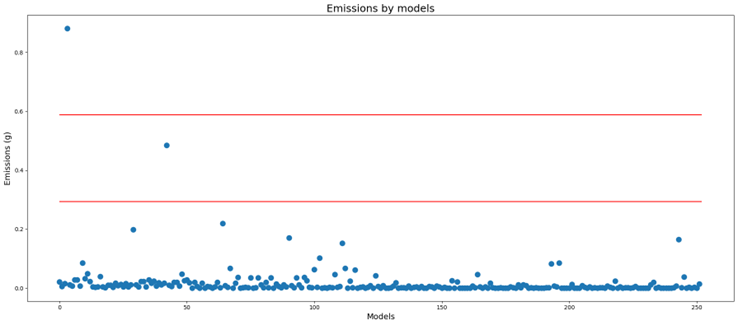
\includegraphics[scale=1.25]{images/nuova-situazione.png}
\end{figure}

Come è possibile notare, i nuovi esperimenti hanno portato a un'ulteriore sbilanciamento nel dataset, in quanto tutti gli esperimenti con DGCF svettano sui risultati degli altri modelli.

Questo si riflette nei risultati ottenuti dai modelli di regressione

\begin{table}[H]
    \centering
    \begin{tabular}{|>{\centering\arraybackslash}m{5cm}|c|c|c|c|}
        \hline
        \textbf{Regressor} & \textbf{MAE} & \textbf{RMSE} & \textbf{MSLE} \\ [10pt]
        \hline
        SVR & 0.0995056 & 0.0161732 & 0.0111161 \\ [10pt]
        \hline
        Decision Tree & 0.0201826 & 0.0037623 & 0.0021361 \\ [10pt]
        \hline
        Random Forest & 0.0236930 & 0.0078052 & 0.0039711 \\ [10pt]
        \hline
        AdaBoost & 0.0311916 & 0.0053061 & 0.0029177 \\ [10pt]
        \hline
    \end{tabular}
    \caption*{Risultati ottenuti}
    \label{tab:results}
\end{table}

\begin{table}[H]
    \centering
    \footnotesize
    \setlength\tabcolsep{0pt}
    \begin{tabularx}{\textwidth}{|X|X|}
        \hline
        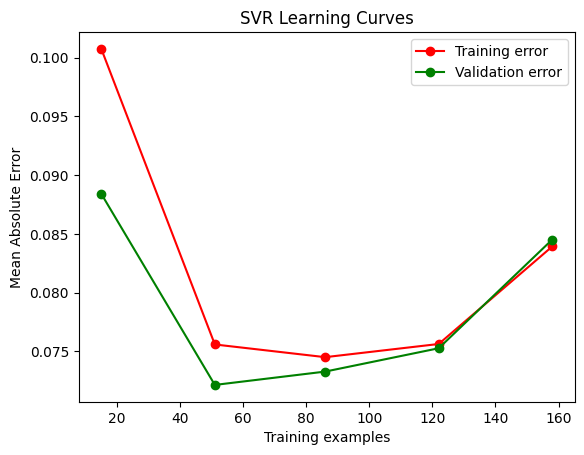
\includegraphics[width=\linewidth, trim=0 0 0 0]{images/SVR_lc2.png} &
        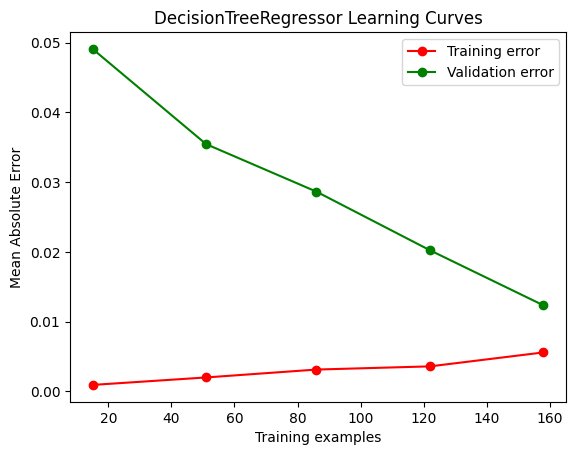
\includegraphics[width=\linewidth, trim=0 0 0 0]{images/DecisionTree_lc2.png} \\
        \hline
        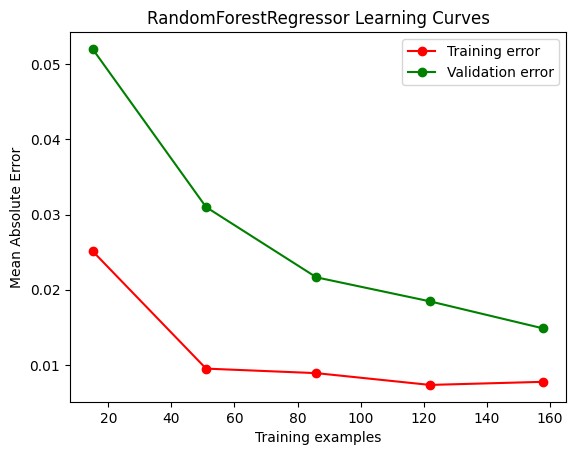
\includegraphics[width=\linewidth, trim=0 0 0 0]{images/RandomForestRegressor_lc2.png} &
        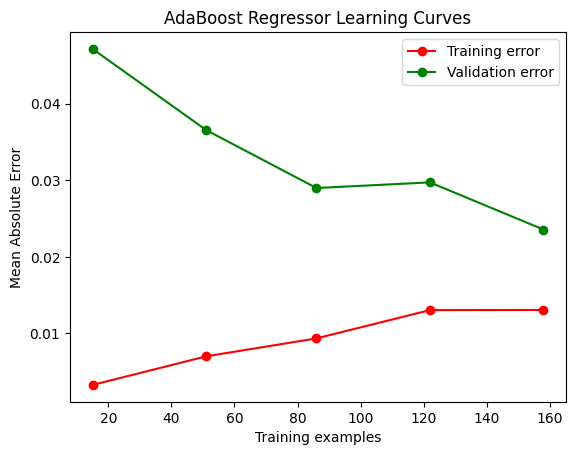
\includegraphics[width=\linewidth, trim=0 0 0 0]{images/AdaBoostRegressor_lc2.png} \\
        \hline
    \end{tabularx}
    \caption{Trade-off con il dataset LFM-1b\_artist\_20U50I}
    \label{tab:emissions_info}
\end{table}


\subsubsection{Dataset Azure}

\noindent Una possibile soluzione è stata quella di eliminare tutti i risultati non prodotti sulla macchina Azure. Le emissioni risultato ancora sbilanciate ma si è riscontrato un leggero miglioramento nei risultati dei modelli di regressione

\begin{figure}[H]
    \centering
    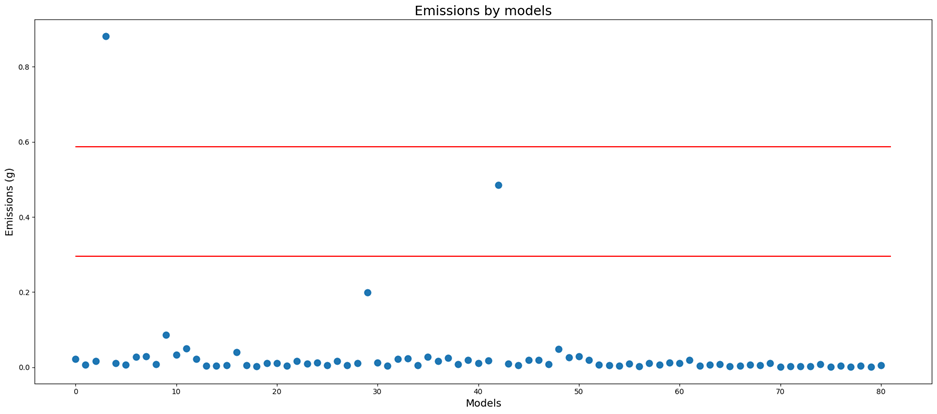
\includegraphics[scale=1]{images/nuova-situazione2.png}
\end{figure}



\begin{table}[H]
    \centering
    \begin{tabular}{|>{\centering\arraybackslash}m{5cm}|c|c|c|c|}
        \hline
        \textbf{Regressor} & \textbf{MAE} & \textbf{RMSE} & \textbf{MSLE} \\ [10pt]
        \hline
        SVR & 0.0923003 & 0.0085932 & 0.0076811 \\ [10pt]
        \hline
        Decision Tree & 0.0165181 & 0.0033569 & 0.0019016 \\ [10pt]
        \hline
        Random Forest & 0.0144149 & 0.0007829 & 0.0005558 \\ [10pt]
        \hline
        AdaBoost & 0.0221310 & 0.0035251 & 0.0020638 \\ [10pt]
        \hline
    \end{tabular}
    \caption*{Risultati ottenuti}
    \label{tab:results}
\end{table}

\begin{table}[H]
    \centering
    \footnotesize
    \setlength\tabcolsep{0pt}
    \begin{tabularx}{\textwidth}{|X|X|}
        \hline
        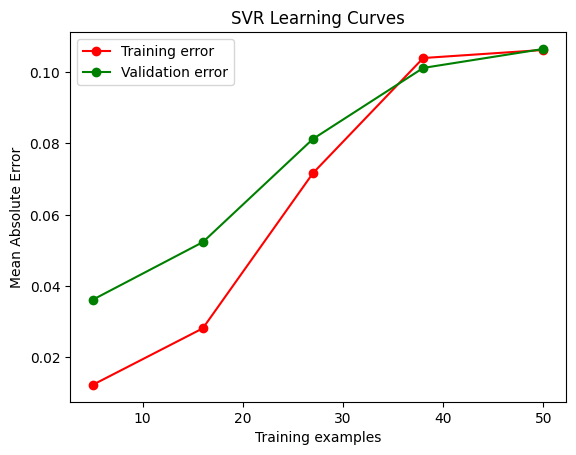
\includegraphics[width=\linewidth, trim=0 0 0 0]{images/SVR_Azure_lc2.png} &
        \includegraphics[width=\linewidth, trim=0 0 0 0]{images/DecisionTree_Azure_lc2.png} \\
        \hline
        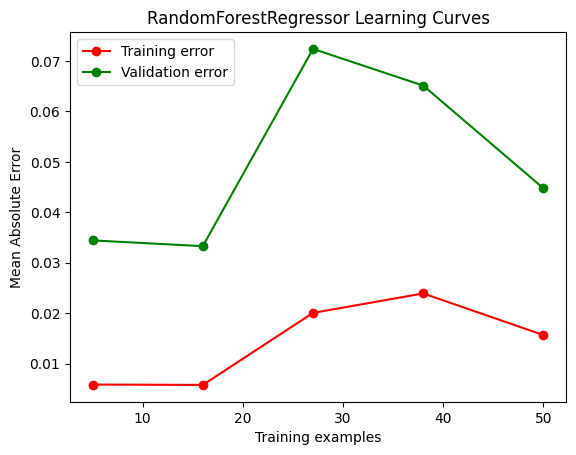
\includegraphics[width=\linewidth, trim=0 0 0 0]{images/RandomForestRegressor_Azure_lc2.png} &
        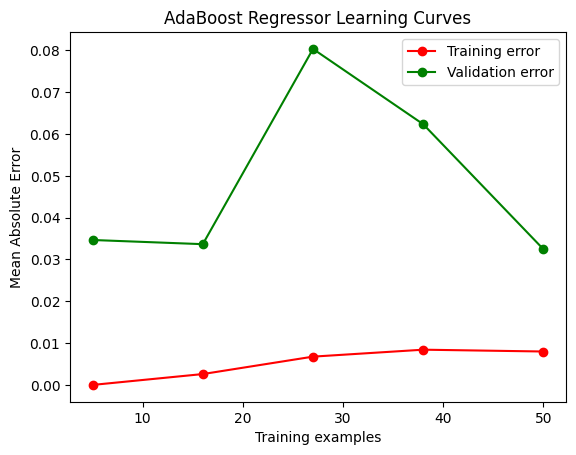
\includegraphics[width=\linewidth, trim=0 0 0 0]{images/AdaBoostRegressor_Azure_lc2.png} \\
        \hline
    \end{tabularx}
    \caption{Trade-off con il dataset LFM-1b\_artist\_20U50I}
    \label{tab:emissions_info}
\end{table}



\subsection{Dataset ridotto}

Per provare a migliorare ancor di più le performance dei modelli di regressione, si è deciso di eliminare tutti gli outlier dal dataset(in questo caso le emissioni più alte). In particolare si sono eliminate 11 emissioni dal dataset completo e 5 dal dataset AZURE.

\subsubsection{Dataset completo}

\begin{figure}[H]
    \centering
    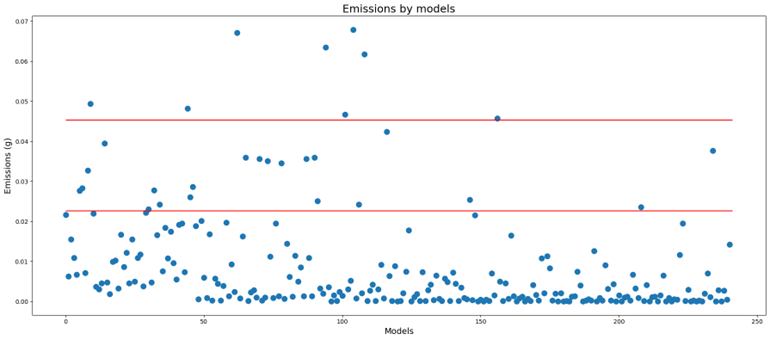
\includegraphics[scale=1.25]{images/nuova-situazione-ridotto.png}
\end{figure}

E' possibile notare un miglior bilanciamento delle emissioni. Per quanto riguarda i modelli, sono stati eseguti addestramenti con diversi split tra training e test set

\textbf{Slit 50/50}


\begin{table}[H]
    \centering
    \begin{tabular}{|>{\centering\arraybackslash}m{5cm}|c|c|c|c|}
        \hline
        \textbf{Regressor} & \textbf{MAE} & \textbf{RMSE} & \textbf{MSLE} \\ [10pt]
        \hline
        SVR & 0.026350 & 0.0008080 & 0.0007787 \\ [10pt]
        \hline
        Decision Tree & 0.0091483 & 0.0003243 & 0.0003048 \\ [10pt]
        \hline
        Random Forest & 0.0073434 & 0.0001388 & 0.00013121 \\ [10pt]
        \hline
        AdaBoost & 0.0115256 & 0.0003340 & 0.0003147 \\ [10pt]
        \hline
    \end{tabular}
    \caption*{Risultati ottenuti}
    \label{tab:results}
\end{table}

//TODO: aggiungere le nuove learning curve se necessario

\textbf{Split 60/40}


\begin{table}[H]
    \centering
    \begin{tabular}{|>{\centering\arraybackslash}m{5cm}|c|c|c|c|}
        \hline
        \textbf{Regressor} & \textbf{MAE} & \textbf{RMSE} & \textbf{MSLE} \\ [10pt]
        \hline
        SVR & 0.0264396 & 0.0007823 & 0.000754 \\ [10pt]
        \hline
        Decision Tree & 0.0079836 & 0.0001961 & 0.0001866 \\ [10pt]
        \hline
        Random Forest & 0.0069729 & 0.0001164 & 0.0001116 \\ [10pt]
        \hline
        AdaBoost & 0.0081044 & 0.0001324 & 0.0001269 \\ [10pt]
        \hline
    \end{tabular}
    \caption*{Risultati ottenuti}
    \label{tab:results}
\end{table}

//TODO: aggiungere le nuove learning curve se necessario

\textbf{Split 70/30}


\begin{table}[H]
    \centering
    \begin{tabular}{|>{\centering\arraybackslash}m{5cm}|c|c|c|c|}
        \hline
        \textbf{Regressor} & \textbf{MAE} & \textbf{RMSE} & \textbf{MSLE} \\ [10pt]
        \hline
        SVR & 0.02635137 & 0.0007884 & 0.0007602 \\ [10pt]
        \hline
        Decision Tree & 0.0072258 & 0.0001427 & 0.0001372 \\ [10pt]
        \hline
        Random Forest & 0.0068948 & 0.0001102 & 0.0001059 \\ [10pt]
        \hline
        AdaBoost & 0.0076783 & 0.0001130 & 0.0001089 \\ [10pt]
        \hline
    \end{tabular}
    \caption*{Risultati ottenuti}
    \label{tab:results}
\end{table}

//TODO: aggiungere le nuove learning curve se necessario


\textbf{Split 80/20}


\begin{table}[H]
    \centering
    \begin{tabular}{|>{\centering\arraybackslash}m{5cm}|c|c|c|c|}
        \hline
        \textbf{Regressor} & \textbf{MAE} & \textbf{RMSE} & \textbf{MSLE} \\ [10pt]
        \hline
        SVR & 0.0270399 & 0.0008109 & 0.0007820 \\ [10pt]
        \hline
        Decision Tree & 0.0067696 & 0.0001287 & 0.0001236 \\ [10pt]
        \hline
        Random Forest & 0.0063234 & 0.0001004 & 0.0000967 \\ [10pt]
        \hline
        AdaBoost & 0.0081434 & 0.0001208 & 0.0001167 \\ [10pt]
        \hline
    \end{tabular}
    \caption*{Risultati ottenuti}
    \label{tab:results}
\end{table}

//TODO: aggiungere le nuove learning curve se necessario



\textbf{Split 90/10}


\begin{table}[H]
    \centering
    \begin{tabular}{|>{\centering\arraybackslash}m{5cm}|c|c|c|c|}
        \hline
        \textbf{Regressor} & \textbf{MAE} & \textbf{RMSE} & \textbf{MSLE} \\ [10pt]
        \hline
        SVR & 0.0266539 & 0.0007763 & 0.0007483 \\ [10pt]
        \hline
        Decision Tree & 0.0056915 & 0.0000799 & 0.0000774 \\ [10pt]
        \hline
        Random Forest & 0.0051378 & 0.0000524 & 0.0000509 \\ [10pt]
        \hline
        AdaBoost & 0.0073941 & 0.00000991 & 0.0000961 \\ [10pt]
        \hline
    \end{tabular}
    \caption*{Risultati ottenuti}
    \label{tab:results}
\end{table}


TODO: aggiungere le nuove learning curve se necessario



\textbf{Conclusioni}

Come si può notare in generale la riduzione del dataset ha portato a miglioramenti. Per quanto riguarda i diversi split si può notare che alcuni modelli performano meglio con alcuni split, altri modelli con altri


\subsubsection{Dataset AZURE}

\begin{figure}[H]
    \centering
    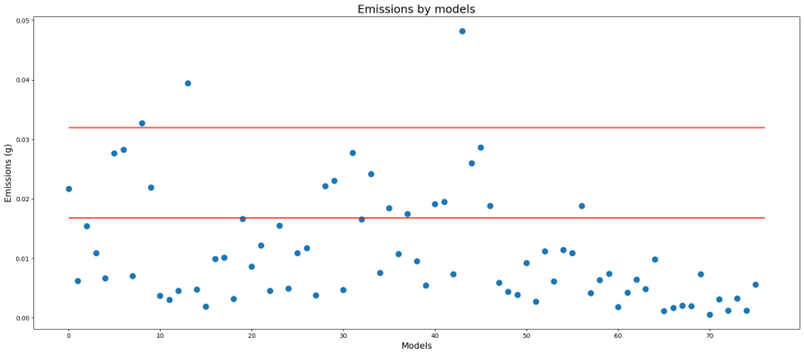
\includegraphics[scale=1.25]{images/nuova-situazione2-ridotto.png}
\end{figure}


E’ possibile notare un miglior bilanciamento delle emissioni. Per quanto riguarda i modelli,
sono stati eseguti addestramenti con diversi split tra training e test set


\textbf{Slit 50/50}


\begin{table}[H]
    \centering
    \begin{tabular}{|>{\centering\arraybackslash}m{5cm}|c|c|c|c|}
        \hline
        \textbf{Regressor} & \textbf{MAE} & \textbf{RMSE} & \textbf{MSLE} \\ [10pt]
        \hline
        SVR & 0.0148003 & 0.0002638 & 0.0002559 \\ [10pt]
        \hline
        Decision Tree & 0.0066692 & 0.0001030 & 0.0000987 \\ [10pt]
        \hline
        Random Forest & 0.0056723 & 0.0000667 & 0.0000644 \\ [10pt]
        \hline
        AdaBoost & 0.0070703 & 0.0001008 & 0.0000975 \\ [10pt]
        \hline
    \end{tabular}
    \caption*{Risultati ottenuti}
    \label{tab:results}
\end{table}

//TODO: aggiungere le nuove learning curve se necessario

\textbf{Split 60/40}


\begin{table}[H]
    \centering
    \begin{tabular}{|>{\centering\arraybackslash}m{5cm}|c|c|c|c|}
        \hline
        \textbf{Regressor} & \textbf{MAE} & \textbf{RMSE} & \textbf{MSLE} \\ [10pt]
        \hline
        SVR & 0.0148974 & 0.000269 & 0.0002609 \\ [10pt]
        \hline
        Decision Tree & 0.0071797 & 0.0001293 & 0.00001239 \\ [10pt]
        \hline
        Random Forest & 0.0049437 & 0.0000621 & 0.0000598 \\ [10pt]
        \hline
        AdaBoost & 0.0059144 & 0.0000805 & 0.0000775 \\ [10pt]
        \hline
    \end{tabular}
    \caption*{Risultati ottenuti}
    \label{tab:results}
\end{table}

//TODO: aggiungere le nuove learning curve se necessario

\textbf{Split 70/30}


\begin{table}[H]
    \centering
    \begin{tabular}{|>{\centering\arraybackslash}m{5cm}|c|c|c|c|}
        \hline
        \textbf{Regressor} & \textbf{MAE} & \textbf{RMSE} & \textbf{MSLE} \\ [10pt]
        \hline
        SVR & 0.0145669 & 0.0002622 & 0.0002543 \\ [10pt]
        \hline
        Decision Tree & 0.0059280 & 0.0000885 & 0.0000851 \\ [10pt]
        \hline
        Random Forest & 0.0057711 & 0.0000790 & 0.000076 \\ [10pt]
        \hline
        AdaBoost & 0.0065205 & 0.0000858 & 0.0000827 \\ [10pt]
        \hline
    \end{tabular}
    \caption*{Risultati ottenuti}
    \label{tab:results}
\end{table}

//TODO: aggiungere le nuove learning curve se necessario


\textbf{Split 80/20}


\begin{table}[H]
    \centering
    \begin{tabular}{|>{\centering\arraybackslash}m{5cm}|c|c|c|c|}
        \hline
        \textbf{Regressor} & \textbf{MAE} & \textbf{RMSE} & \textbf{MSLE} \\ [10pt]
        \hline
        SVR & 0.0137841 & 0.0002431 & 0.0002356 \\ [10pt]
        \hline
        Decision Tree & 0.0070346 & 0.0001177 & 0.0001133 \\ [10pt]
        \hline
        Random Forest & 0.0061398 & 0.0001047 & 0.0001007 \\ [10pt]
        \hline
        AdaBoost & 0.0073228 & 0.0001225 & 0.0001181 \\ [10pt]
        \hline
    \end{tabular}
    \caption*{Risultati ottenuti}
    \label{tab:results}
\end{table}

//TODO: aggiungere le nuove learning curve se necessario



\textbf{Split 90/10}

\begin{table}[H]
    \centering
    \begin{tabular}{|>{\centering\arraybackslash}m{5cm}|c|c|c|c|}
        \hline
        \textbf{Regressor} & \textbf{MAE} & \textbf{RMSE} & \textbf{MSLE} \\ [10pt]
        \hline
        SVR & 0.0193509 & 0.0003821 & 0.0003712 \\ [10pt]
        \hline
        Decision Tree & 0.0055465 & 0.0000506 & 0.0000494 \\ [10pt]
        \hline
        Random Forest & 0.0032249 & 0.000021 & 0.0000207 \\ [10pt]
        \hline
        AdaBoost & 0.0050706 & 0.0000415 & 0.00000406 \\ [10pt]
        \hline
    \end{tabular}
    \caption*{Risultati ottenuti}
    \label{tab:results}
\end{table}


TODO: aggiungere le nuove learning curve se necessario



\textbf{Conclusioni}

Come si può notare in generale la riduzione del dataset ha portato a miglioramenti. Per quanto riguarda i diversi split si può notare che alcuni modelli performano meglio con alcuni split, altri modelli con altri


\subsubsection{Dataset AZURE}

\begin{figure}[H]
    \centering
    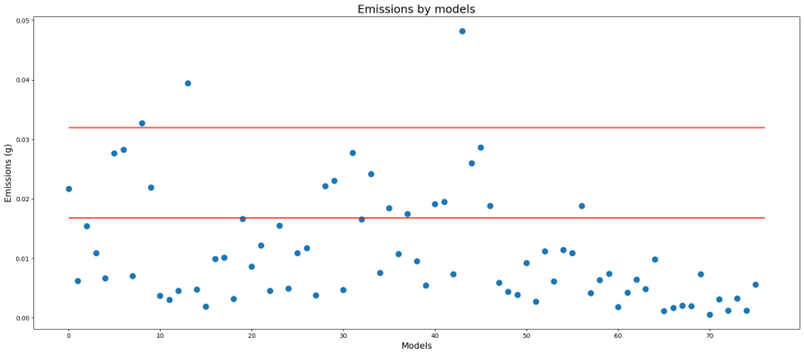
\includegraphics[scale=1.25]{images/nuova-situazione2-ridotto.png}
\end{figure}
    \newpage
    \bibliography{bibliography}
\end{document}
